\documentclass[11pt,a4paper]{article}

\usepackage[T1]{fontenc}
\usepackage[utf8]{inputenc}
% \usepackage{lmodern}
\usepackage[margin=2.3cm]{geometry}
\usepackage{amsmath,amssymb}
\usepackage{siunitx}
\usepackage{booktabs}
\usepackage{array}
\usepackage{tabularx}
\usepackage{caption}
\usepackage{xcolor}
\usepackage{tikz}
\usetikzlibrary{decorations.pathmorphing,arrows.meta,positioning,calc}
\usepackage[european,siunitx,RPvoltages]{circuitikz}
\usepackage{listings}
\usepackage{fancyhdr}
\usepackage[hidelinks]{hyperref}

\ctikzset{voltage dir=EF, inductor=american, transistors/scale=1.4}

\sisetup{per-mode=symbol}

\lstset{
  basicstyle=\ttfamily\footnotesize,
  breaklines=true,
  columns=fullflexible,
  keepspaces=true,
  frame=single,
  framerule=0.3pt,
  numbers=left,
  numberstyle=\tiny\color{gray},
  numbersep=6pt,
  commentstyle=\color{gray!80!black},
  morecomment=[l]{\%},
  language=Matlab,
  showstringspaces=false
}

\newcommand{\Rev}{Rev.~00}
\newcommand{\RevDate}{2026-09-19}
\newcommand{\DocTitle}{\texttt{mos\_simple\_2th}: simplified power MOSFET loss model with separate thermal ports}

\newcommand{\Eon}{E_{\mathrm{on}}}
\newcommand{\Eoff}{E_{\mathrm{off}}}
\newcommand{\Err}{E_{\mathrm{rr}}}
\newcommand{\Rdson}{R_{\mathrm{DS(on)}}}
\newcommand{\Vdc}{V_{\mathrm{dc}}}
\newcommand{\Tj}{T_{\mathrm{j}}}
\newcommand{\Ht}{H_{\mathrm{t}}}
\newcommand{\Hd}{H_{\mathrm{d}}}
\newcommand{\ih}{i_{\mathrm{h}}}
\newcommand{\idh}{i_{\mathrm{dh}}}
\newcommand{\vh}{v_{\mathrm{h}}}
\newcommand{\taus}{\tau_{\mathrm{s}}}
\newcommand{\taup}{\tau_{\mathrm{p}}}
\newcommand{\tauo}{\tau_{\mathrm{o}}}
\newcommand{\code}[1]{\texttt{#1}}

\pagestyle{fancy}
\fancyhf{}
\fancyhead[L]{\small\texttt{mos\_simple\_2th} -- \Rev}
\fancyhead[R]{\small\RevDate}
\fancyfoot[C]{\small\thepage}
\renewcommand{\headrulewidth}{0.3pt}

\title{\DocTitle\\[0.6em]{\large \Rev\ -- \RevDate}}
\author{D.~Bagnara}
\date{}

\begin{document}
\maketitle
\thispagestyle{fancy}

\begin{abstract}
\noindent
This note describes the Simscape language component \code{mos\_simple\_2th}, a
simplified power MOSFET model for loss estimation and nominal-value thermal
dimensioning. It is the MOSFET counterpart of \code{igbt\_simple\_2th}: same
port interface, same single-point switching energies scaled with current and
voltage, same continuous sample-and-hold states and the same
energy-to-power conversion towards two thermal ports, $\Ht$ for the channel
and $\Hd$ for the antiparallel diode. The differences are those imposed by the
device: a bidirectional resistive channel with third-quadrant conduction, a
body diode that carries the current only during the dead time in synchronous
rectification, zero-voltage turn-on, and a diode that is physically on the
same chip as the channel.
\end{abstract}

\begin{table}[h]
\centering
\caption*{Revision history}
\begin{tabular}{@{}lll@{}}
\toprule
Rev. & Date & Description \\
\midrule
00 & \RevDate & First issue. \\
\bottomrule
\end{tabular}
\end{table}

\tableofcontents

\section{Scope}

The component computes, in a circuit simulation with ideal-switching
semiconductors, the conduction and switching losses of a power MOSFET and of
its antiparallel diode and delivers them, separately, to two thermal
conserving ports. The switching transients are not resolved: the model is not
meant for snubber, overvoltage or EMI studies (for those the switching-dynamics
model \code{mos\_dyn} exists). The purpose is a nominal-value dimensioning:
average and cyclic losses, junction temperature ripple over the output
fundamental, heatsink verification.

The modelling choices are the same as in \code{igbt\_simple\_2th}, documented
in \code{igbt\_simple\_doc}; this note repeats only what is needed to read
the source and dwells on what is different for a MOSFET. A user of the IGBT
block can replace it with the MOSFET block without changing the surrounding
model.

\section{Interface}

\begin{table}[htbp]
\centering
\caption{Ports, inputs and outputs.}
\label{tab:ports}
\begin{tabularx}{\textwidth}{@{}llX@{}}
\toprule
Name & Type & Meaning \\
\midrule
\code{D}, \code{S} & electrical & Drain and source. Positive current $i$ from D to S, terminal voltage $v = v_\mathrm{D} - v_\mathrm{S}$. \\
\code{Ht} & thermal & Channel chip: conduction $v\,i_\mathrm{t}$ plus $\Eon$, $\Eoff$. \\
\code{Hd} & thermal & Diode chip: conduction $v\,i_\mathrm{d}$ plus $\Err$. \\
\code{G} & input, \si{\volt} & Gate signal. Channel on for $g > V_\mathrm{th}$; switching events at $V_\mathrm{th} \pm V_\mathrm{hyst}$. \\
\code{Pt}, \code{Pd} & output, \si{\watt} & Instantaneous losses delivered to $\Ht$ and $\Hd$ (conduction plus averaged switching power). \\
\code{Pt\_flt}, \code{Pd\_flt} & output, \si{\watt} & The same, filtered with $\tauo$ for display; not used by the thermal ports. \\
\code{it}, \code{id} & output, \si{\ampere} & Channel and diode currents. In blocking they carry the leakage $v\,G_\mathrm{off}$. \\
\bottomrule
\end{tabularx}
\end{table}

\begin{table}[htbp]
\centering
\caption{Parameters. Defaults are placeholders for a generic \SI{1200}{\volt}/\SI{300}{\ampere} SiC MOSFET half-bridge at $T_\mathrm{vj} = \SI{125}{\celsius}$ and must be replaced with datasheet values.}
\label{tab:params}
\small
\begin{tabularx}{\textwidth}{@{}llrX@{}}
\toprule
Name & Symbol & Default & Meaning \\
\midrule
\multicolumn{4}{@{}l}{\emph{Conduction}} \\
\code{Rds\_on}  & $\Rdson$ & \SI{5}{\milli\ohm} & Channel on-state resistance at $T_\mathrm{ref}$. \\
\code{alpha\_R} & $\alpha_R$ & \SI{0}{\per\kelvin} & Linear temperature coefficient of $\Rdson$; 0 = fixed value at $T_\mathrm{ref}$. \\
\code{T\_ref}   & $T_\mathrm{ref}$ & \SI{398.15}{\kelvin} & Reference junction temperature of $\Rdson$ (\SI{125}{\celsius}). \\
\code{Vf}       & $V_\mathrm{f}$ & \SI{2.6}{\volt} & Diode threshold voltage. \\
\code{Rd}       & $R_\mathrm{d}$ & \SI{5}{\milli\ohm} & Diode differential resistance. \\
\addlinespace
\multicolumn{4}{@{}l}{\emph{Gate}} \\
\code{Vth}   & $V_\mathrm{th}$ & \SI{4}{\volt} & Gate-source threshold. \\
\code{Vhyst} & $V_\mathrm{hyst}$ & \SI{1}{\volt} & Half hysteresis band of the switching events. \\
\addlinespace
\multicolumn{4}{@{}l}{\emph{Switching energies, single point}} \\
\code{Eon\_ref}, \code{Eoff\_ref} & $\Eon^\ast$, $\Eoff^\ast$ & \SI{12}{\milli\joule}, \SI{6}{\milli\joule} & Channel energies at $I_\mathrm{ref}$, $V_\mathrm{ref}$. \\
\code{Err\_ref} & $\Err^\ast$ & \SI{1}{\milli\joule} & Diode recovery energy at $I_\mathrm{ref}$, $V_\mathrm{ref}$. \\
\code{Ic\_ref}, \code{Vdc\_ref} & $I_\mathrm{ref}$, $V_\mathrm{ref}$ & \SI{300}{\ampere}, \SI{600}{\volt} & Reference conditions of the energies. \\
\code{k\_i}, \code{k\_v} & $k_i$, $k_v$ & 1, 1 & Current and voltage exponents of $\Eon$, $\Eoff$. \\
\code{k\_id}, \code{k\_vd} & $k_{id}$, $k_{vd}$ & 1, 1 & Current and voltage exponents of $\Err$. \\
\addlinespace
\multicolumn{4}{@{}l}{\emph{Numerical}} \\
\code{V\_rr\_th} & $V_\mathrm{rr,th}$ & \SI{50}{\volt} & Voltage level detecting the recovery event. \\
\code{i\_eps}    & $i_\varepsilon$ & \SI{10}{\milli\ampere} & Reverse-conduction detection level of $\idh$. \\
\code{Goff}      & $G_\mathrm{off}$ & \SI{1e-6}{\per\ohm} & Off-state conductance. \\
\code{tau\_s}    & $\taus$ & \SI{1}{\micro\second} & Sample-and-hold time constant. \\
\code{tau\_p}    & $\taup$ & \SI{200}{\micro\second} & Switching-energy averaging time constant. \\
\code{tau\_o}    & $\tauo$ & \SI{1}{\milli\second} & Display filter of \code{Pt\_flt}, \code{Pd\_flt}. \\
\bottomrule
\end{tabularx}
\end{table}

\section{Conduction model}

\begin{figure}[htbp]
\centering
\begin{circuitikz}[scale=1.15, transform shape]
  % terminals
  \draw (0,5.2) node[ocirc, label=above:\code{D}] (D) {}
        to[short, i=$i$] (0,4.4);
  \draw (0,0.8) -- (0,0) node[ocirc, label=below:\code{S}] (S) {};
  % top and bottom buses
  \draw (0,4.4) -- (-2,4.4) (0,4.4) -- (2,4.4);
  \draw (0,0.8) -- (-2,0.8) (0,0.8) -- (2,0.8);
  % channel branch
  \draw (-2,4.4) to[cspst, l=$g>V_\mathrm{th}$, name=SW] (-2,3.0)
        to[R, l=$\Rdson(\Tj)$, i=$i_\mathrm{t}$] (-2,0.8);
  % diode branch (anode at S)
  \draw (2,0.8) to[D, l_=$V_\mathrm{f}+R_\mathrm{d}$, i<_=$i_\mathrm{d}$] (2,4.4);
  % voltage arrow
  \draw (0.9,4.4) to[open, v=$v$] (0.9,0.8);
  % thermal ports
  \draw[-{Stealth[length=2mm]}, thick, red!65!black,
        decorate, decoration={snake, amplitude=0.35mm, segment length=2mm, post length=1.5mm}]
        (-2.35,1.9) -- ++(-1.4,0) node[left, black] {$\Ht$: $v\,i_\mathrm{t}+\Eon+\Eoff$};
  \draw[-{Stealth[length=2mm]}, thick, red!65!black,
        decorate, decoration={snake, amplitude=0.35mm, segment length=2mm, post length=1.5mm}]
        (2.35,3.7) -- ++(1.4,0) node[right, black] {$\Hd$: $v\,i_\mathrm{d}+\Err$};
\end{circuitikz}
\caption{Equivalent circuit of the component. The channel is a bidirectional resistance in series with an ideal switch; the diode conducts for $v<-V_\mathrm{f}$. The two branches dissipate towards two distinct thermal ports.}
\label{fig:model}
\end{figure}

\subsection{Channel}

The channel is a linear resistance, on for $g > V_\mathrm{th}$ and bidirectional:
\begin{equation}
i_\mathrm{t} =
\begin{cases}
 v / R_\mathrm{on}(\Tj) & g > V_\mathrm{th} \\
 v\, G_\mathrm{off}     & \text{otherwise},
\end{cases}
\qquad
R_\mathrm{on}(\Tj) = \Rdson\,\bigl[1 + \alpha_R\,(\Tj - T_\mathrm{ref})\bigr],
\label{eq:channel}
\end{equation}
with $\Tj$ read from the $\Ht$ port. With the default $\alpha_R = 0$ the
resistance is the fixed \SI{125}{\celsius} value, as in the IGBT model, and the
electrical and thermal networks are decoupled. A non-zero $\alpha_R$ closes the
electro-thermal loop, which for a MOSFET is worth doing because $\Rdson$
varies by a factor 2 to 2.5 between \SI{25}{\celsius} and \SI{150}{\celsius}
in silicon and by 1.4 to 1.7 in SiC (Section~\ref{sec:param}).

\subsection{Diode}

The diode is a threshold voltage plus a differential resistance:
\begin{equation}
i_\mathrm{d} =
\begin{cases}
 (v + V_\mathrm{f}) / R_\mathrm{d} & v < -V_\mathrm{f} \\
 v\, G_\mathrm{off}                & \text{otherwise}.
\end{cases}
\label{eq:diode}
\end{equation}
Unlike the IGBT model, where $R_\mathrm{d}$ was a numerical conditioning
term, here both $V_\mathrm{f}$ and $R_\mathrm{d}$ are physical: the body diode
of a SiC MOSFET has a threshold around \SIrange{2.5}{3}{\volt} and a slope
resistance comparable to $\Rdson$, and the two together determine how the
current splits during the dead time and how much the diode dissipates.

\subsection{Third-quadrant operation}
\label{sec:3q}

The two branches are in parallel and the channel resistance has no
preferential direction, so third-quadrant conduction requires no additional
logic. With $i<0$ and the gate on, $v = i\,R_\mathrm{on}$ is a few hundred
millivolts and the diode is off: the current flows in the channel and the loss
is charged to $\Ht$. With the gate off the current flows in the diode at
$v = -V_\mathrm{f} + i\,R_\mathrm{d}$ and the loss is charged to $\Hd$. The
diode is therefore active only during the dead times and whenever
$|i|\,R_\mathrm{on} > V_\mathrm{f}$, when it shares the current with the channel
exactly as in the real device.

\section{Switching losses}

\subsection{Scaling law}

Each energy is a single datasheet point scaled with the commutated current
$I$ and the blocking voltage $V$:
\begin{equation}
E = E^\ast \left(\frac{I}{I_\mathrm{ref}}\right)^{k} \left(\frac{V}{V_\mathrm{ref}}\right)^{k_v}.
\label{eq:scaling}
\end{equation}
The exponents are parameters, with $k = k_v = 1$ by default so that the block
reproduces the bilinear law of the IGBT model. For a MOSFET a sub-linear
current exponent is often the better fit, in particular for $\Eoff$, which at
low current is dominated by the output-capacitance energy
$E_\mathrm{oss}$ and does not go to zero with $I$ (Section~\ref{sec:param}).
The quantities $I$ and $V$ are not taken at the switching instant, where the
solver already sees the post-transition values, but from the held states of
Section~\ref{sec:sh}.

\subsection{Attribution to the two chips}

$\Eon$ and $\Eoff$ are dissipated in the channel of the device that switches,
and are added to the accumulator $E_\mathrm{t}$ at the rising and falling edges
of its own gate. $\Err$ is dissipated in the diode of \emph{this} device when
the \emph{complementary} switch of the leg turns on. That instant is not
visible from the gate; it is detected locally, as in the IGBT model, as the
rising edge of the terminal voltage above $V_\mathrm{rr,th}$, and the energy is
added to the accumulator $E_\mathrm{d}$.

$\Eon$ and $\Err$ are not the same energy counted twice. When the channel turns
on against a conducting diode, the recovery current of that diode flows
through the channel at full voltage and its loss is part of the datasheet
$\Eon$ of the switching device; the loss inside the recovering diode is
$\Err$. Both are used, provided the datasheet $\Eon$ was measured with the
same diode that freewheels in the application (Section~\ref{sec:param}).

\subsection{Sample-and-hold states}
\label{sec:sh}

Three continuous states with time constant $\taus$ store the pre-commutation
quantities. The channel current, used for $\Eon$ and $\Eoff$:
\begin{equation}
\taus\,\dot{\ih} =
\left\{\begin{array}{l@{\qquad}l@{\qquad}l}
 i_\mathrm{t} - \ih & g > V_\mathrm{th} & \text{(track, channel on)} \\
 -\ih              & v < -V_\mathrm{f} & \text{(flush, diode conducting)} \\
 0                 & \text{otherwise}   & \text{(hold, blocking)}
\end{array}\right.
\label{eq:ih}
\end{equation}
At turn-off $\ih$ is the current being switched off. At turn-on it is the
current switched off one period earlier if the device has been blocking since,
which is the current about to be switched on; it is zero if the diode of the
device has conducted in the meantime, because the channel then closes at
zero voltage. The flush branch is the MOSFET-specific addition: in the IGBT
model $\ih$ only tracked and held, and a turn-on with the own diode conducting
was charged $\Eon$ at the previous turn-off current.

The blocking voltage, used by all three energies:
\begin{equation}
\taus\,\dot{\vh} =
\begin{cases}
 v - \vh & g < V_\mathrm{th} \;\wedge\; v > 0 \\
 0       & \text{otherwise}.
\end{cases}
\label{eq:vh}
\end{equation}
The reverse-current magnitude, used for $\Err$:
\begin{equation}
\taus\,\dot{\idh} =
\left\{\begin{array}{l@{\qquad}l@{\qquad}l}
 -i - \idh & i < -i_\varepsilon & \text{(track, reverse conduction)} \\
 -\idh     & g > V_\mathrm{th} \;\wedge\; i > i_\varepsilon & \text{(flush, forward channel)} \\
 0         & \text{otherwise} & \text{(hold, blocking)}
\end{array}\right.
\label{eq:idh}
\end{equation}
This is the second MOSFET-specific change. The IGBT version tracked the
\emph{diode} current, $v<-V_\mathrm{f}$, and flushed whenever the transistor
was gated on. In a MOSFET with synchronous rectification the reverse current
is in the channel for most of the period and in the diode only during the dead
time before the recovery, typically \SIrange{0.2}{1}{\micro\second} for SiC,
too short for a tracker with $\taus\approx\SI{1}{\micro\second}$ to settle.
The state therefore tracks the total reverse current, whichever path it takes:
what is recovered is the current that the diode carries at the end of the dead
time, and that is the load current regardless of how it was shared a moment
before. The flush condition is restricted to \emph{forward} channel
conduction, so that gating the channel on in the third quadrant does not
erase the held value.

\subsection{Events}

The three events are a single \code{when}/\code{elsewhen} chain, because two
separate \code{when} clauses updating the same event variable are rejected by
the compiler, and the branches are mutually exclusive by construction. With
$[x]^+ = (x+|x|)/2 = \max(x,0)$:
\begin{align}
g \uparrow (V_\mathrm{th}+V_\mathrm{hyst}):\quad &
E_\mathrm{t} \leftarrow E_\mathrm{t} + \Eon^\ast
\left(\frac{[\ih]^+}{I_\mathrm{ref}}\right)^{k_i}
\left(\frac{|\vh|}{V_\mathrm{ref}}\right)^{k_v}
\label{eq:evon}\\
g \downarrow (V_\mathrm{th}-V_\mathrm{hyst}):\quad &
E_\mathrm{t} \leftarrow E_\mathrm{t} + \Eoff^\ast
\left(\frac{[\ih]^+}{I_\mathrm{ref}}\right)^{k_i}
\left(\frac{|\vh|}{V_\mathrm{ref}}\right)^{k_v}
\label{eq:evoff}\\
v \uparrow V_\mathrm{rr,th}:\quad &
E_\mathrm{d} \leftarrow E_\mathrm{d} + \Err^\ast
\left(\frac{|\idh|}{I_\mathrm{ref}}\right)^{k_{id}}
\left(\frac{|\vh|}{V_\mathrm{ref}}\right)^{k_{vd}}.
\label{eq:everr}
\end{align}
The positive part $[\ih]^+$ replaces the $|\ih|$ of the IGBT model: a channel
that is switched with negative current commutates with its own diode, at
zero voltage, and neither $\Eon$ nor $\Eoff$ is generated. At the turn-off of a
device carrying forward current the gate edge and the voltage edge coincide;
the chain executes only the first branch, and the $\Err$ branch is skipped,
which is correct since $\idh$ has been flushed anyway.

\subsection{Behaviour over the two half periods}

Figure~\ref{fig:timing} follows one switching period of the device in the half
period of the output fundamental in which it carries reverse current
(synchronous rectification). Table~\ref{tab:halfperiods} summarises both half
periods.

\begin{figure}[htbp]
\centering
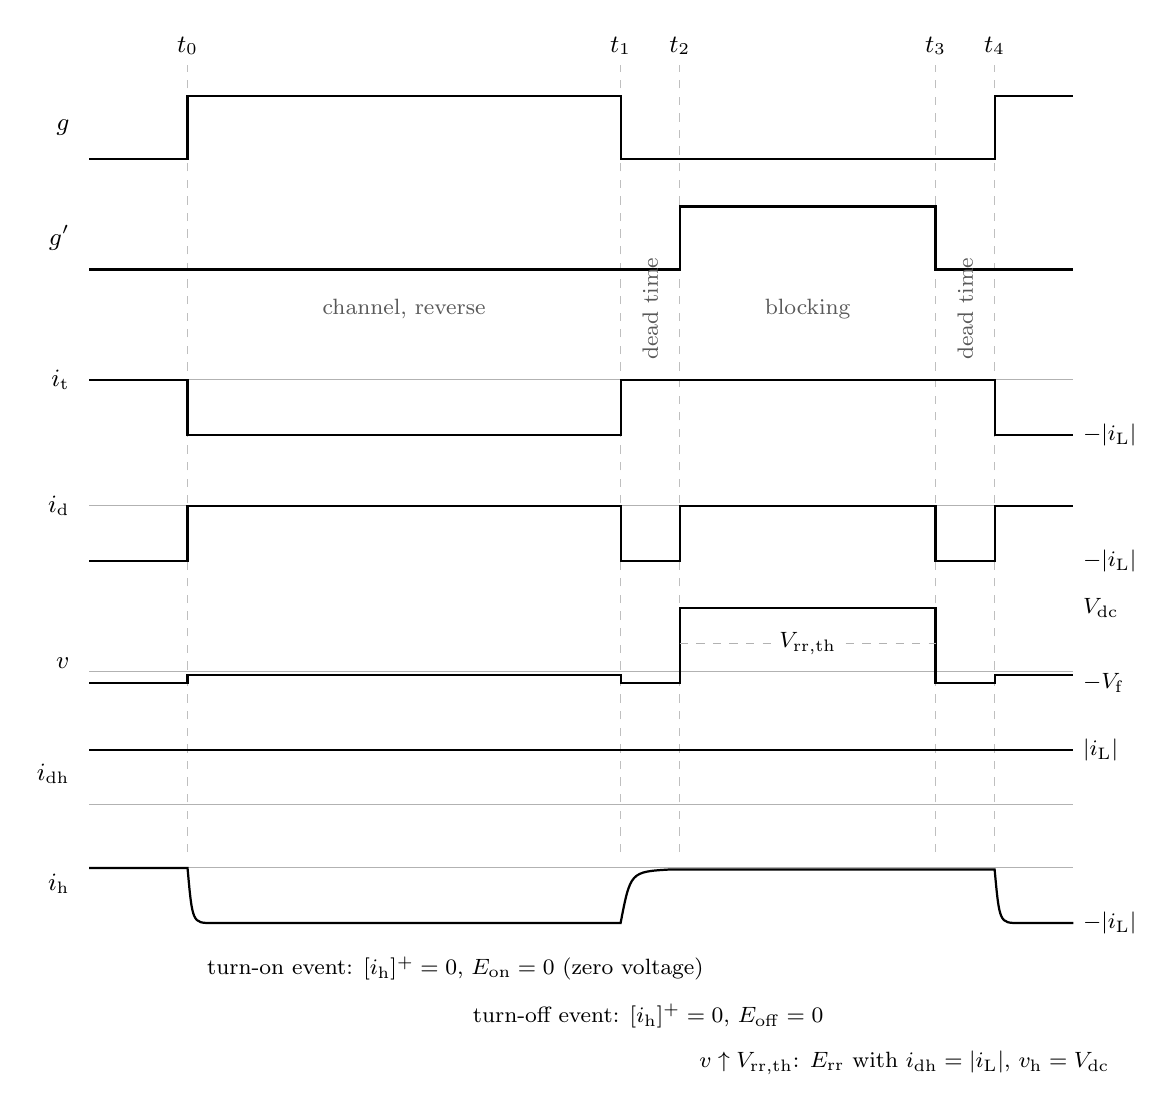
\begin{tikzpicture}[x=1.25cm, y=1cm, >=Stealth, font=\small]
  % time markers
  \def\ta{1} \def\tb{5.4} \def\tc{6.0} \def\td{8.6} \def\te{9.2} \def\tf{10}
  \foreach \t in {\ta,\tb,\tc,\td,\te}
    \draw[gray!50, dashed] (\t,-0.4) -- (\t,9.6);
  \node[above] at (\ta,9.6) {$t_0$};
  \node[above] at (\tb,9.6) {$t_1$};
  \node[above] at (\tc,9.6) {$t_2$};
  \node[above] at (\td,9.6) {$t_3$};
  \node[above] at (\te,9.6) {$t_4$};
  % row labels helper
  \newcommand{\rowlabel}[2]{\node[left] at (-0.1,#1) {#2};}
  % g (this device)
  \rowlabel{8.8}{$g$}
  \draw[thick] (0,8.4) -- (\ta,8.4) -- (\ta,9.2) -- (\tb,9.2) -- (\tb,8.4) -- (\te,8.4) -- (\te,9.2) -- (\tf,9.2);
  % g' (complementary)
  \rowlabel{7.4}{$g'$}
  \draw[thick] (0,7.0) -- (\tc,7.0) -- (\tc,7.8) -- (\td,7.8) -- (\td,7.0) -- (\tf,7.0);
  % i_t
  \rowlabel{5.6}{$i_\mathrm{t}$}
  \draw[gray!60] (0,5.6) -- (\tf,5.6);
  \draw[thick] (0,5.6) -- (\ta,5.6) -- (\ta,4.9) -- (\tb,4.9) -- (\tb,5.6) -- (\te,5.6) -- (\te,4.9) -- (\tf,4.9);
  \node[right, font=\footnotesize] at (\tf,4.9) {$-|i_\mathrm{L}|$};
  % i_d
  \rowlabel{4.0}{$i_\mathrm{d}$}
  \draw[gray!60] (0,4.0) -- (\tf,4.0);
  \draw[thick] (0,3.3) -- (\ta,3.3) -- (\ta,4.0) -- (\tb,4.0) -- (\tb,3.3) -- (\tc,3.3)
        -- (\tc,4.0) -- (\td,4.0) -- (\td,3.3) -- (\te,3.3) -- (\te,4.0) -- (\tf,4.0);
  \node[right, font=\footnotesize] at (\tf,3.3) {$-|i_\mathrm{L}|$};
  % v
  \rowlabel{2.0}{$v$}
  \draw[gray!60] (0,1.9) -- (\tf,1.9);
  \draw[thick] (0,1.75) -- (\ta,1.75) -- (\ta,1.85) -- (\tb,1.85) -- (\tb,1.75) -- (\tc,1.75)
        -- (\tc,2.7) -- (\td,2.7) -- (\td,1.75) -- (\te,1.75) -- (\te,1.85) -- (\tf,1.85);
  \node[right, font=\footnotesize] at (\tf,2.7) {$\Vdc$};
  \node[right, font=\footnotesize] at (\tf,1.75) {$-V_\mathrm{f}$};
  \draw[gray!60, dashed] (\tc,2.25) -- (\td,2.25);
  \node[font=\footnotesize, fill=white, inner sep=1pt] at (7.3,2.25) {$V_\mathrm{rr,th}$};
  % i_dh
  \rowlabel{0.6}{$\idh$}
  \draw[gray!60] (0,0.2) -- (\tf,0.2);
  \draw[thick] (0,0.9) -- (\tf,0.9);
  \node[right, font=\footnotesize] at (\tf,0.9) {$|i_\mathrm{L}|$};
  % i_h
  \rowlabel{-0.8}{$\ih$}
  \draw[gray!60] (0,-0.6) -- (\tf,-0.6);
  \draw[thick] (0,-0.6) -- (\ta,-0.6) .. controls (\ta+0.05,-1.3) .. (\ta+0.25,-1.3) -- (\tb,-1.3)
        .. controls (\tb+0.1,-0.65) .. (\tb+0.5,-0.62) -- (\te,-0.62) .. controls (\te+0.05,-1.3) .. (\te+0.25,-1.3) -- (\tf,-1.3);
  \node[right, font=\footnotesize] at (\tf,-1.3) {$-|i_\mathrm{L}|$};
  % event annotations
  \node[align=left, font=\footnotesize, anchor=north west] at (\ta+0.1,-1.6)
        {turn-on event: $[\ih]^+=0$, $\Eon=0$ (zero voltage)};
  \node[align=left, font=\footnotesize, anchor=north west] at (\tb-1.6,-2.2)
        {turn-off event: $[\ih]^+=0$, $\Eoff=0$};
  \node[align=left, font=\footnotesize, anchor=north west] at (\tc+0.1,-2.8)
        {$v\uparrow V_\mathrm{rr,th}$: $\Err$ with $\idh=|i_\mathrm{L}|$, $\vh=\Vdc$};
  % interval labels
  \node[font=\footnotesize, gray!70!black] at ({(\ta+\tb)/2},6.5) {channel, reverse};
  \node[font=\footnotesize, gray!70!black] at ({(\tc+\td)/2},6.5) {blocking};
  \node[font=\footnotesize, gray!70!black, rotate=90] at ({(\tb+\tc)/2},6.5) {dead time};
  \node[font=\footnotesize, gray!70!black, rotate=90] at ({(\td+\te)/2},6.5) {dead time};
\end{tikzpicture}
\caption{One switching period in the half period with reverse load current. $t_0$: channel on, current moves from the diode to the channel. $t_1$: channel off, current back to the diode. $t_2$: complementary switch on, recovery, $v$ rises to $\Vdc$. $t_3$: complementary switch off, dead time. $t_4$: next turn-on at zero voltage. $\idh$ tracks $|i|$ through channel and diode alike and holds during blocking; $\ih$ is negative or flushed, so no channel energy is generated.}
\label{fig:timing}
\end{figure}

\begin{table}[htbp]
\centering
\caption{Held states and generated energies in the two half periods of the output fundamental.}
\label{tab:halfperiods}
\small
\begin{tabularx}{\textwidth}{@{}lXX@{}}
\toprule
 & Forward current ($i>0$) & Reverse current ($i<0$) \\
\midrule
Channel on & carries $i$; $\ih$ tracks $i>0$; $\idh$ flushed & carries $i$; $\ih$ tracks $i<0$; $\idh$ tracks $|i|$ \\
Own turn-off & $\Eoff(\ih>0,\vh)$; $v$ rises, $\Err$ branch skipped (chain) & $\Eoff = 0$; current to own diode \\
Dead time after own turn-off & device blocks, $\vh$ tracks $\Vdc$; $\ih$, $\idh$ hold & own diode conducts; $\idh$ tracks, $\ih$ flushes \\
Complementary turn-on & no edge on this device & $v\uparrow V_\mathrm{rr,th}$: $\Err(\idh=|i|,\vh)$ \\
Complementary on & blocking; complementary diode inactive & blocking; $\vh$ tracks $\Vdc$; $\idh$ holds $|i|$ \\
Dead time before own turn-on & complementary diode conducts; device blocks; $\ih$ holds $i>0$ & own diode conducts; $\idh$ tracks \\
Own turn-on & $\Eon(\ih>0,\vh)$: hard switching & $\Eon = 0$: $\ih \le 0$, zero-voltage turn-on \\
\bottomrule
\end{tabularx}
\end{table}

At the zero crossings of the load current the sign of $i$ changes inside a
switching period and one event of each kind is evaluated with a partially
tracked or partially flushed state. The error is one switching event per
fundamental half period and is irrelevant for a thermal dimensioning.

\section{Energy-to-power conversion and thermal ports}

The event variables $E_\mathrm{t}$ and $E_\mathrm{d}$ are staircases. Each is
converted to a power by a first-order lag with time constant $\taup$:
\begin{equation}
\taup\,\dot{E}_\mathrm{lp} = E - E_\mathrm{lp}, \qquad
P_\mathrm{sw} = \frac{E - E_\mathrm{lp}}{\taup} = \dot{E}_\mathrm{lp}.
\label{eq:lag}
\end{equation}
Since $P_\mathrm{sw}$ is the derivative of $E_\mathrm{lp}$ and
$E_\mathrm{lp}\to E$ after the last event, the energy delivered to the thermal
port equals the accumulated energy: the lag only spreads each step over a few
$\taup$, without changing its integral. The total losses are
\begin{equation}
P_\mathrm{t} = v\,i_\mathrm{t} + \frac{E_\mathrm{t}-E_\mathrm{lp,t}}{\taup},
\qquad
P_\mathrm{d} = v\,i_\mathrm{d} + \frac{E_\mathrm{d}-E_\mathrm{lp,d}}{\taup},
\end{equation}
and are bound to the thermal ports with the sign convention of the thermal
domain, positive $Q$ flowing into the component: $Q_\mathrm{t} = -P_\mathrm{t}$
and $Q_\mathrm{d} = -P_\mathrm{d}$. $\taup$ must be a few switching periods,
so that the thermal network sees a smooth power, and much shorter than the
smallest thermal time constant of interest.

\subsection{Two ports on one chip}
\label{sec:onechip}

In an IGBT module the transistor and the freewheeling diode are two chips
with two thermal impedances, and the two ports give two junction
temperatures. In a MOSFET the body diode is the drain-body junction of the
same die: channel and diode losses heat the same silicon. In that case the
two ports must be connected to the \emph{same} junction node, feeding a single
$Z_\mathrm{th(j-c)}$ (Figure~\ref{fig:thermal}); the split between $\Ht$ and
$\Hd$ remains available through \code{Pt} and \code{Pd} as a loss breakdown
and for the cross-check against the vendor's loss calculator, but it is not two
temperatures. The ports are kept separate for the modules that do have a
discrete antiparallel diode chip (SiC MOSFET with SiC Schottky, silicon MOSFET
with external fast diode); there $V_\mathrm{f}$, $R_\mathrm{d}$ and $\Err^\ast$
describe the external chip, whose lower threshold keeps the body diode off, and
$\Hd$ gets its own $Z_\mathrm{th}$.

\begin{figure}[htbp]
\centering
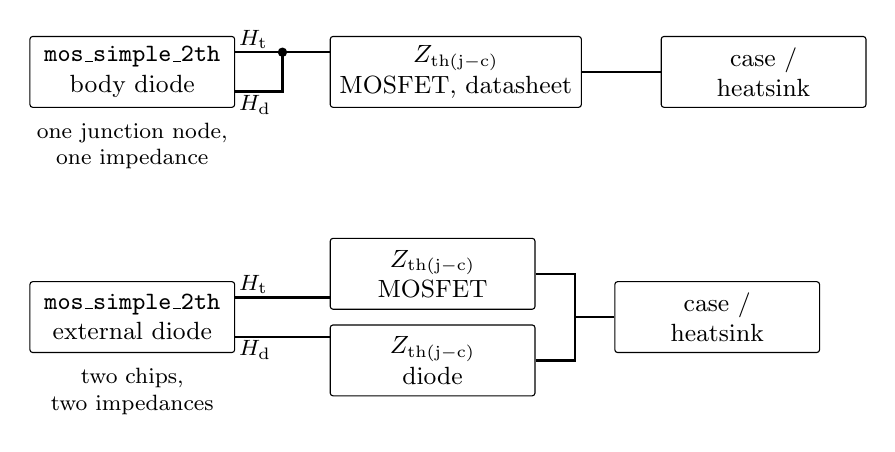
\begin{tikzpicture}[>=Stealth, font=\small, node distance=8mm]
  \tikzset{blk/.style={draw, rounded corners=1pt, minimum width=2.6cm, minimum height=0.9cm, align=center}}
  % left: body diode
  \node[blk] (M1) {\code{mos\_simple\_2th}\\ body diode};
  \node[blk, right=1.2cm of M1] (Z1) {$Z_\mathrm{th(j-c)}$\\ MOSFET, datasheet};
  \node[blk, right=1.0cm of Z1] (C1) {case /\\ heatsink};
  \draw[thick] ($(M1.east)+(0,0.25)$) node[above right, font=\footnotesize, inner sep=1pt] {$\Ht$} -- ++(0.6,0) coordinate (j1) -- (Z1.west |- j1);
  \draw[thick] ($(M1.east)+(0,-0.25)$) node[below right, font=\footnotesize, inner sep=1pt] {$\Hd$} -- ++(0.6,0) -- (j1);
  \draw[thick] (Z1) -- (C1);
  \node[fill=black, circle, inner sep=1.2pt] at (j1) {};
  \node[below=2pt of M1, font=\footnotesize, align=center] {one junction node,\\ one impedance};
  % right: external diode
  \node[blk, below=2.2cm of M1] (M2) {\code{mos\_simple\_2th}\\ external diode};
  \node[blk, right=1.2cm of M2, yshift=0.55cm] (Z2t) {$Z_\mathrm{th(j-c)}$\\ MOSFET};
  \node[blk, right=1.2cm of M2, yshift=-0.55cm] (Z2d) {$Z_\mathrm{th(j-c)}$\\ diode};
  \node[blk, right=1.0cm of Z2t, yshift=-0.55cm] (C2) {case /\\ heatsink};
  \draw[thick] ($(M2.east)+(0,0.25)$) node[above right, font=\footnotesize, inner sep=1pt] {$\Ht$} -- (Z2t.west |- {$(M2.east)+(0,0.25)$}) ;
  \draw[thick] ($(M2.east)+(0,-0.25)$) node[below right, font=\footnotesize, inner sep=1pt] {$\Hd$} -- (Z2d.west |- {$(M2.east)+(0,-0.25)$});
  \draw[thick] (Z2t.east) -- ++(0.5,0) |- (C2.west);
  \draw[thick] (Z2d.east) -- ++(0.5,0) |- (C2.west);
  \node[below=2pt of M2, font=\footnotesize, align=center] {two chips,\\ two impedances};
\end{tikzpicture}
\caption{Connection of the thermal ports. Top: intrinsic body diode, one junction. Bottom: discrete antiparallel diode chip, two junctions.}
\label{fig:thermal}
\end{figure}

\section{Outputs}

\code{Pt} and \code{Pd} are the powers actually delivered to the thermal ports.
\code{Pt\_flt} and \code{Pd\_flt} are the same signals through a further lag
$\tauo$, for scopes and for the average-loss readout; they do not enter the
thermal network, so $\tauo$ can be raised for readability without altering the
junction temperature. The current outputs \code{it}, \code{id} carry the
leakage $v\,G_\mathrm{off}$ while blocking, of the order of a milliampere at
\SI{1}{\kilo\volt}; if they are integrated for a charge balance this offset
must be subtracted.

\section{Reference circuit}

The parameters and the timing of Figure~\ref{fig:timing} refer to the
half-bridge leg of Figure~\ref{fig:hb}, which is also the datasheet test
circuit for the switching energies. The load current $i_\mathrm{L}$ is positive
out of the switch node; with $i_\mathrm{L}>0$ the upper device works in the
forward-current column of Table~\ref{tab:halfperiods} and the lower one in the
reverse-current column.

\begin{figure}[htbp]
\centering
\begin{circuitikz}[scale=1.1, transform shape]
  % dc link
  \draw (0,0) to[battery2, l_=$\Vdc$, invert] (0,7);
  \draw (0,7) -- (6,7);
  \draw (0,0) -- (6,0);
  \draw (2.5,7) to[C, l=$C$] (2.5,3.6) to[C, l=$C$] (2.5,0);
  % devices
  \draw (6,6.4) node[nigfete, bodydiode, anchor=D] (T1) {};
  \draw (6,2.6) node[nigfete, bodydiode, anchor=D] (T2) {};
  \draw (6,7) to[short, i=$i_1$] (T1.D);
  \draw (T1.S) -- (6,3.6);
  \draw (6,3.6) to[short, i=$i_2$] (T2.D);
  \draw (T2.S) -- (6,0);
  \draw (T1.G) node[left] {$g_1$};
  \draw (T2.G) node[left] {$g_2$};
  \node at ($(T1.D)+(1.1,0.35)$) {$\mathrm{T}_1$};
  \node at ($(T2.D)+(1.1,0.35)$) {$\mathrm{T}_2$};
  % load
  \draw (6,3.6) to[L, l=$L$, i=$i_\mathrm{L}$] (2.5,3.6);
  % voltages
  \draw (T1.D) -- ++(2.4,0) coordinate (a1);
  \draw (T1.S) -- ++(2.4,0) coordinate (b1);
  \draw (a1) to[open, v=$v_1$] (b1);
  \draw (T2.D) -- ++(2.4,0) coordinate (a2);
  \draw (T2.S) -- ++(2.4,0) coordinate (b2);
  \draw (a2) to[open, v=$v_2$] (b2);
\end{circuitikz}
\caption{Half-bridge reference leg. Each device is one instance of the component, gate signals $g_1$, $g_2$ complementary with dead time.}
\label{fig:hb}
\end{figure}

\section{Parameterisation from the datasheet}
\label{sec:param}

\paragraph{Channel.} $\Rdson$ is the typical value at the gate voltage of the
application and at $T_\mathrm{ref}$, read from the $\Rdson(\Tj)$ curve, not the
\SI{25}{\celsius} headline value. If the electro-thermal loop is closed,
$\alpha_R$ is the secant slope between two datasheet temperatures around the
operating point, e.g. between \SI{100}{\celsius} and \SI{150}{\celsius},
normalised to the value at $T_\mathrm{ref}$; typical values around
\SI{125}{\celsius} are \SIrange{5e-3}{7e-3}{\per\kelvin} for silicon and
\SIrange{2.5e-3}{3.5e-3}{\per\kelvin} for SiC. The linear law is adequate
within about \SI{\pm 40}{\kelvin} of $T_\mathrm{ref}$.

\paragraph{Diode.} $V_\mathrm{f}$ and $R_\mathrm{d}$ are the intercept and
slope of a straight line fitted to the body-diode characteristic at
$T_\mathrm{ref}$, with the gate at its \emph{off} voltage, between roughly
$0.3\,I_\mathrm{nom}$ and $I_\mathrm{nom}$. For SiC the characteristic depends
on the negative gate bias; use the value of the application. With a discrete
antiparallel diode, fit that diode instead.

\paragraph{Switching energies.} $\Eon^\ast$, $\Eoff^\ast$ are read at
$I_\mathrm{ref}$, $V_\mathrm{ref}$, $T_\mathrm{ref}$ and at the external gate
resistance of the application; the dependence on $R_\mathrm{G}$ is strong for
SiC and is not modelled. The test circuit matters more than for an IGBT: most
MOSFET datasheets measure $\Eon$ in a half-bridge with the body diode of the
complementary device as freewheeling diode, some with an external SiC Schottky.
Only the first is consistent with a leg of two identical MOSFETs; the second
underestimates $\Eon$ by the recovery-induced term. $\Err^\ast$ is the
body-diode recovery energy, often listed as $E_\mathrm{rec}$ or given through
$Q_\mathrm{rr}$, in which case $\Err^\ast \approx V_\mathrm{ref}\,Q_\mathrm{rr}$
is the usual estimate; for a SiC body diode it is small and mostly capacitive.

\paragraph{Exponents.} With $k_i = k_v = 1$ the block behaves as
\code{igbt\_simple\_2th}. If the datasheet gives $E(I)$ curves, a fit over the
operating range typically returns $k_i \approx 1$ for $\Eon$,
$k_i \approx \numrange{0.6}{0.9}$ for $\Eoff$ and, for the voltage,
$k_v \approx \numrange{1.2}{1.5}$ for $\Eon$ and $\approx\numrange{1.0}{1.3}$
for $\Eoff$. Since the model has one pair of exponents for both channel
energies, choose them on the energy that dominates at the operating point,
or split the difference. For a SiC body diode $k_{id} \approx \numrange{0.3}{0.5}$
reflects the weak current dependence of a mainly capacitive recovery.

\paragraph{Numerical parameters.} $\taus$ must be shorter than about one third
of the shortest on-time and of the dead time, otherwise the trackers do not
settle; \SI{1}{\micro\second} suits IGBT-like dead times, SiC legs with
\SIrange{200}{500}{\nano\second} dead time need \SIrange{0.1}{0.2}{\micro\second}.
$V_\mathrm{rr,th}$ must exceed the largest on-state voltage of both branches and
stay well below the minimum dc-link voltage; \SI{50}{\volt} is adequate for any
device above \SI{600}{\volt}. $\taup$ between two and five switching periods.
$i_\varepsilon$ must exceed the leakage $\Vdc\,G_\mathrm{off}$.

\paragraph{Thermal network.} $Z_\mathrm{th(j-c)}$ of the MOSFET in Foster form
from the datasheet, connected as in Figure~\ref{fig:thermal}; then
$R_\mathrm{th(c-s)}$ per module and the heatsink. For a body-diode device the
datasheet may list a separate $Z_\mathrm{th}$ for the diode: it refers to the
same chip in diode operation and is not a second path; use the MOSFET one and
tie the ports.

\section{Validity limits}

\begin{itemize}
  \item Ideal switching: no $\mathrm{d}v/\mathrm{d}t$, $\mathrm{d}i/\mathrm{d}t$,
        overshoot or recovery current. Use \code{mos\_dyn} for those.
  \item Single-point energies with power-law scaling; no dependence on
        $R_\mathrm{G}$ and, for the energies, on temperature. All parameters are
        meant at \SI{125}{\celsius}.
  \item $\Rdson$ temperature dependence linear and optional; diode
        characteristic fixed.
  \item The dead-time loss of the body diode is modelled through its conduction
        drop; the additional loss of a SiC body diode due to bipolar degradation
        is not.
  \item $\Eon$ at the current zero crossings of the load uses a partially
        settled $\ih$: one switching event per fundamental half period is
        misestimated.
  \item Short on-times, below $3\taus$, leave $\idh$ partially flushed and
        generate a small spurious $\Err$ at the device's own turn-off.
  \item Recovery detection assumes that a rising edge of $v$ above
        $V_\mathrm{rr,th}$ is caused by the complementary switch. In topologies
        where the device voltage rises for other reasons (resonant transitions,
        dc-link steps) the detection must be reviewed.
  \item With the intrinsic body diode the two thermal ports are one junction:
        see Section~\ref{sec:onechip}.
\end{itemize}

\section{Differences with respect to \code{igbt\_simple\_2th}}

\begin{table}[htbp]
\centering
\caption{Summary of the differences between the two components.}
\label{tab:diff}
\small
\begin{tabularx}{\textwidth}{@{}lXX@{}}
\toprule
 & \code{igbt\_simple\_2th} & \code{mos\_simple\_2th} \\
\midrule
Transistor conduction & $V_\mathrm{CE,sat}$ fixed, $R_\mathrm{on}$ numerical, unidirectional & $\Rdson(\Tj)$ resistive, bidirectional \\
Diode conduction & $V_\mathrm{f}$ fixed, $R_\mathrm{d}$ numerical & $V_\mathrm{f} + R_\mathrm{d}$ both physical \\
Third quadrant & diode only & channel when gated, diode in dead time \\
$\ih$ & track / hold & track / flush while own diode conducts / hold \\
$\idh$ & tracks diode current, flushed while gated on & tracks total reverse current, flushed only in forward channel conduction \\
Channel energies & $|\ih|$ & $[\ih]^+$: none in the third quadrant \\
Scaling & bilinear & power laws, exponents as parameters (default bilinear) \\
Thermal ports & two chips, two junctions & one junction for body-diode devices, two for discrete diode \\
Outputs & \code{Pt}, \code{Pd} (plus user additions) & \code{Pt}, \code{Pd}, \code{Pt\_flt}, \code{Pd\_flt}, \code{it}, \code{id} \\
\bottomrule
\end{tabularx}
\end{table}

\appendix
\section{Source listing}

\lstinputlisting{mos_simple_2th.ssc}

\end{document}
